\section{Prise en main de l'application}
\subsection{Organisation de l'application}
\begin{wrapfigure}[18]{r}[0pt]{0.5\textwidth}
  \vspace{-10pt}
  \label{Menu de navigation}
  \centering
  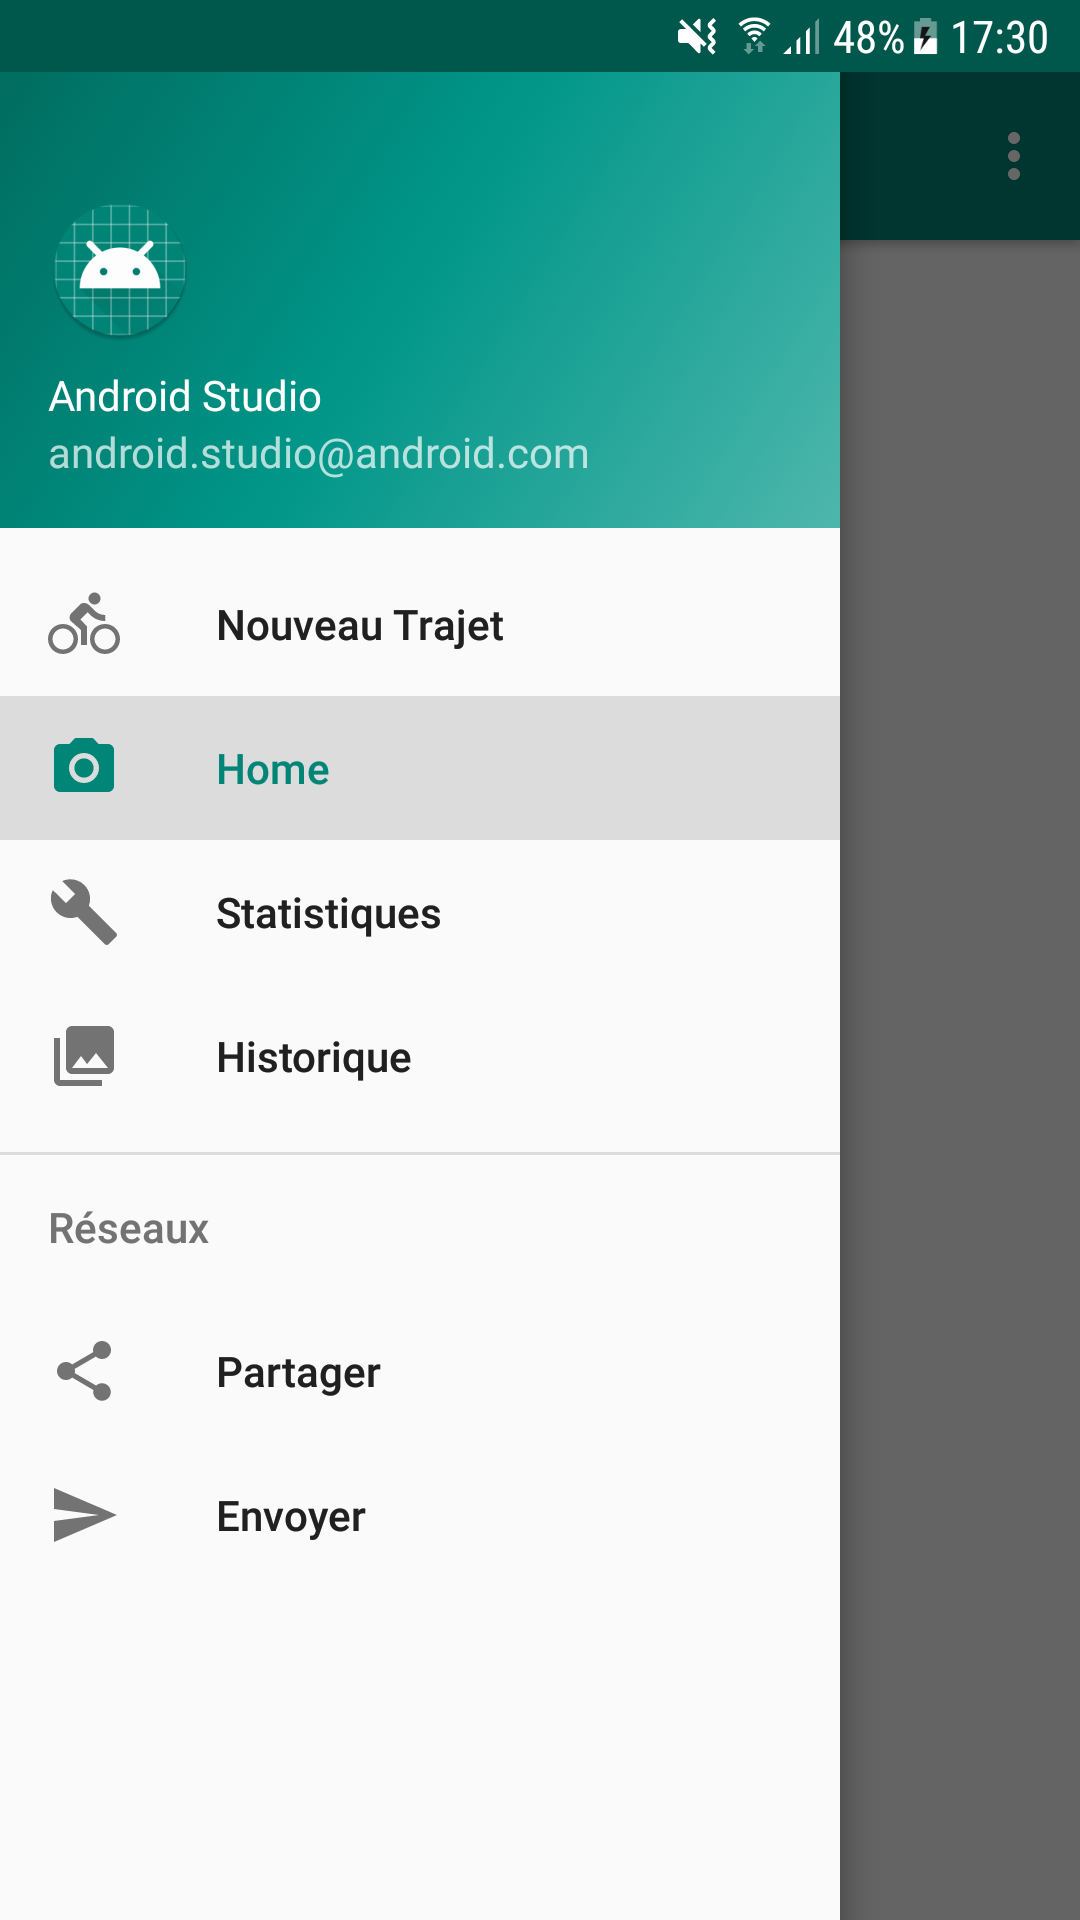
\includegraphics[scale=0.13]{images/navigation-menu.png}
  \caption{Capture d'écran du menu de navigation}
\end{wrapfigure}
L'application se rapproche beaucoup d'une application android standard. Elle possède une page d'accueil vide à notre stade de développement mais
elle est censée contenir à terme les derniers trajets effectués et partagés par nos amis dans l'application.

Un menu de navigation est accessible depuis le bouton en haut à gauche de l'écran ou en faisant glisser le doigt de gauche à droite de l'écran.
Ce menu permet d'accéder aux différentes fonctionnalités du logiciel. Ce menu devait également afficher notre nom d'utilisateur et
possiblement un icône pour nous représenter.

Les onglets effectifs sont les onglets "Nouveau Trajet" et "Historique". Les autres n'ont pas pu être développés.
\vspace{30pt}
\subsection{Onglet "Nouveau Trajet"}
Cet onglet est la partie principale de l'application. Il contient une carte dynamique (google map) et un bouton. Lorsqu'on clique sur ce
bouton, on lance alors la création d'un nouveau trajet. Cela se remarque au bouton qui a changé de texte et de fonction. Il permet
désormais d'indiquer la fin du trajet. De plus, la carte affiche maintenant un point nous représentant. Dès lors, lorsqu'on bouge
le GPS détecte le mouvement et transmet un nouveau point à la carte. Notre position change donc et la suite de ces points affiche un chemin visible
sur la carte.

Une fois le trajet réalisé, on clique sur le bouton en bas de l'écran pour le terminer. Ceci a pour effet de faire apparaître une
petite fenêtre en superposition de la carte. Ce "pop-up" contient une zone de texte et un bouton. Il nous permet de saisir un nom pour
le trajet. Puis, le trajet s'enregistre sur le téléphone et on peut créer un autre trajet.
\begin{figure}[ht]
  \label{Nouveau trajet}
  \centering
  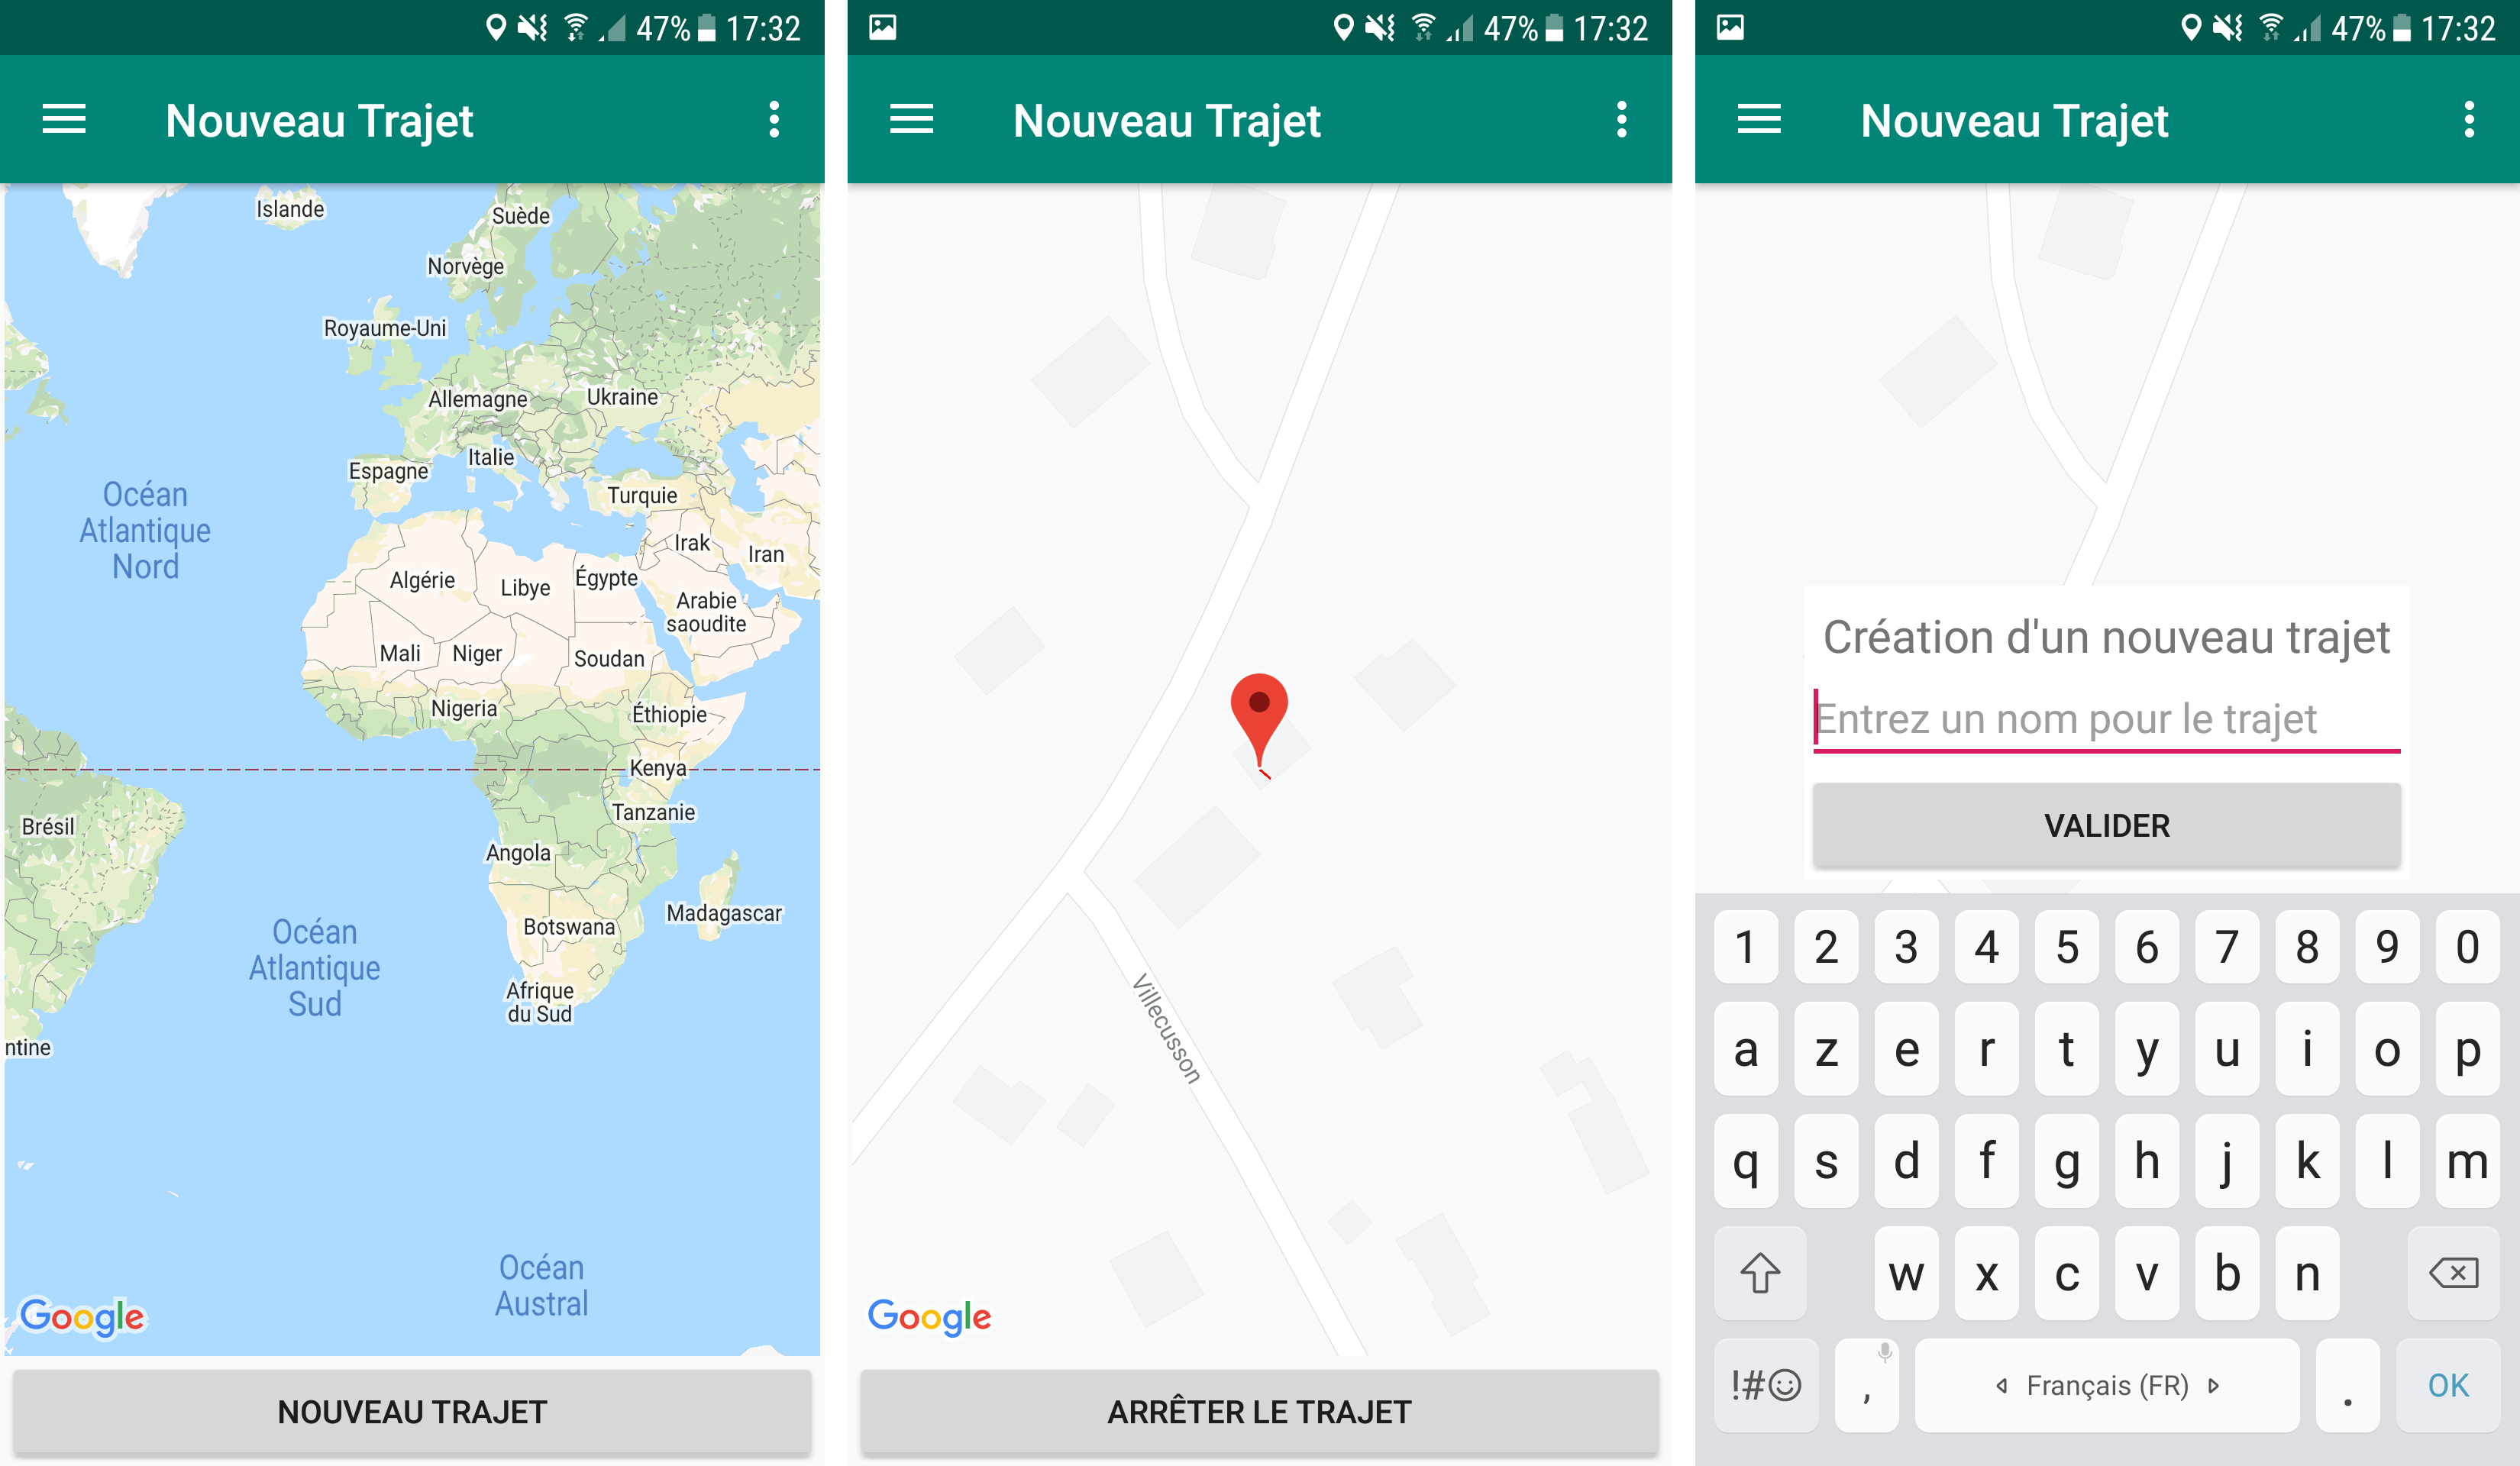
\includegraphics[scale=0.11]{images/nouveau-trajet.png}
  \caption{Multiples captures d'écrans lors d'un nouveau trajet}
\end{figure}

\subsection{Onglet "Historique"}
Cet onglet contient l'ensemble des trajets effectués et enregistrés. Ils s'affichent du plus récent au plus vieux. Chaque trajet est représenté
par une "card", un conteneur composé du nom du trajet, de sa date de création, de sa durée et d'une capture d'écran de la carte prise au moment
de sa création. Si il y a trop de trajets et qu'ils ne rentrent pas tous dans l'écran, on peut les faire défiler grâce à une barre de défilement
en faisant glisser son doigt de bas en haut. Chaque "card" est cliquable et emmène vers une page dédiée au trajet.
\begin{figure}[ht]
  \label{Historique}
  \centering
  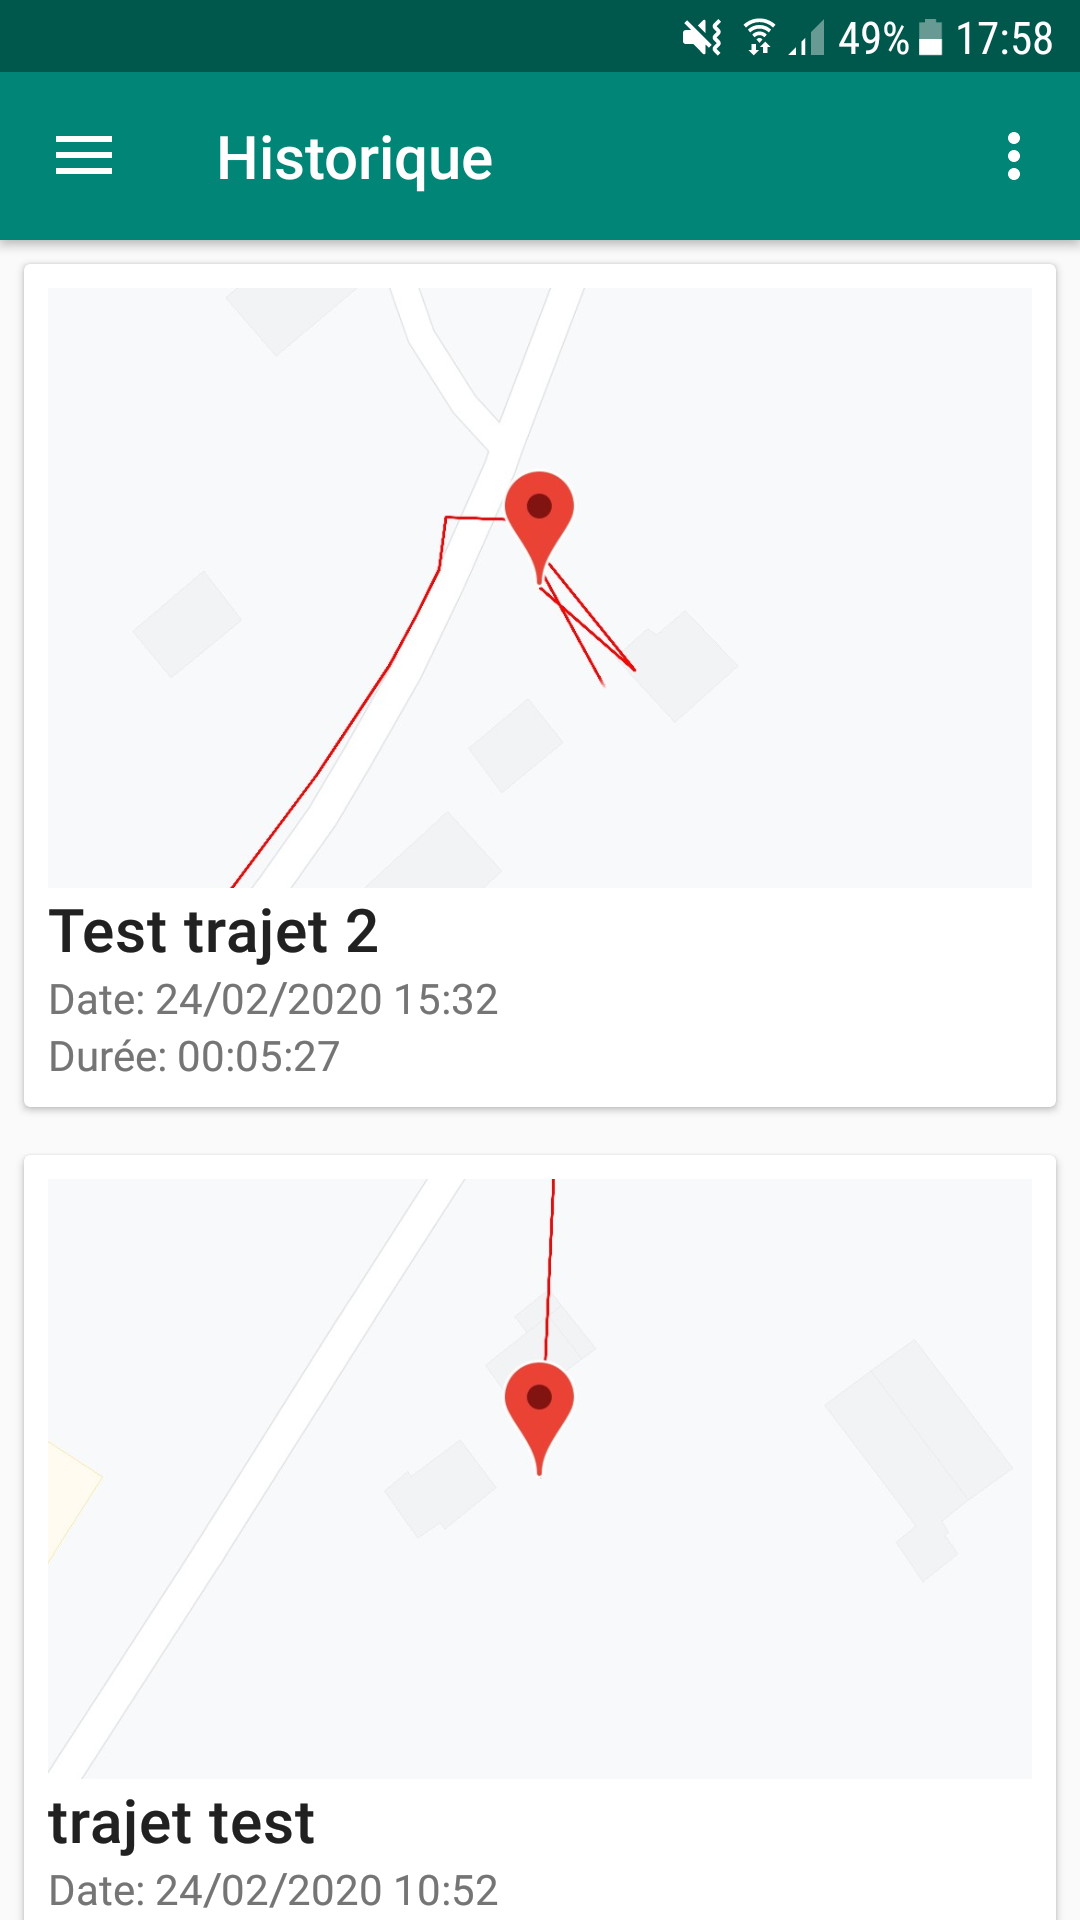
\includegraphics[scale=0.13]{images/historique.png}
  \caption{Capture d'écran de l'historique}
\end{figure}

\subsection{Page "Trajet"}
\begin{wrapfigure}[6]{r}[0pt]{0.5\textwidth}
  \vspace{-50pt}
  \label{Trajet}
  \centering
  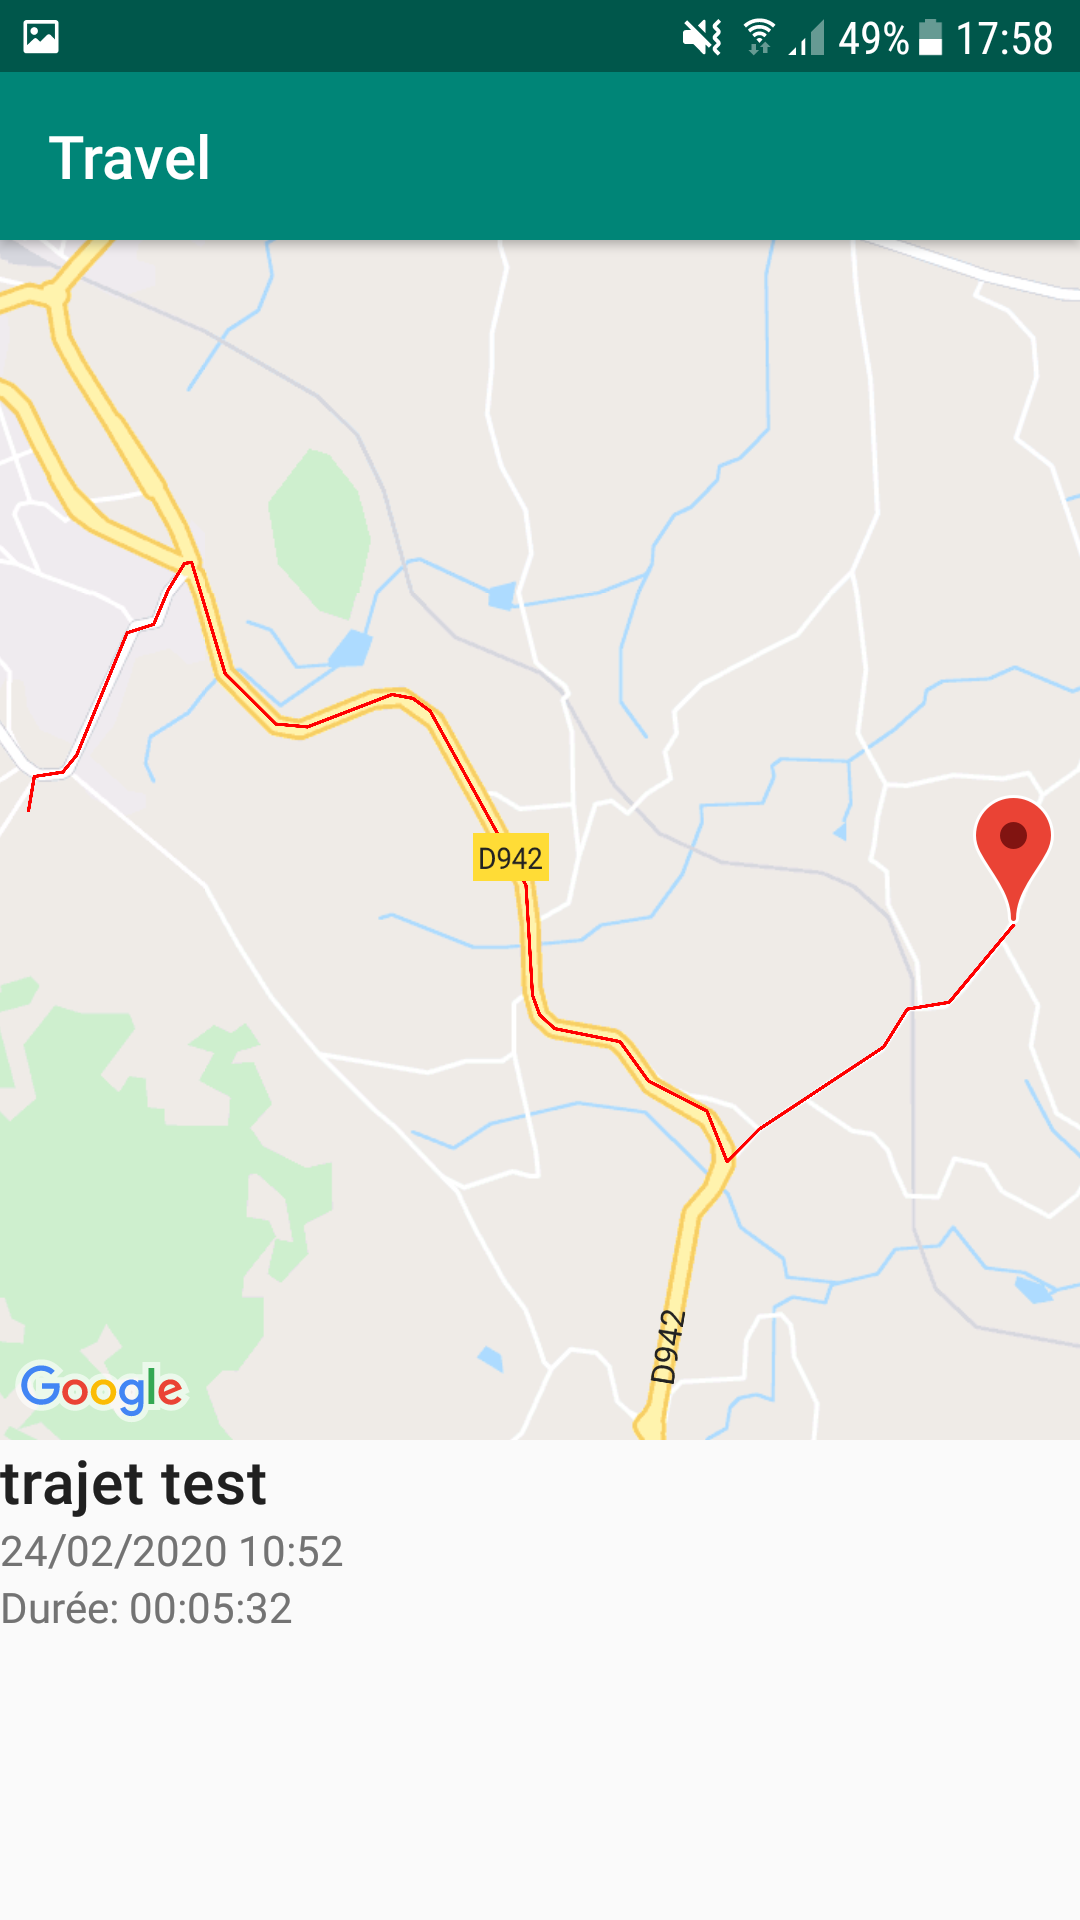
\includegraphics[scale=0.13]{images/travel.png}
  \caption{Capture d'écran d'une page d'un trajet}
\end{wrapfigure}
Une page de trajet s'affiche lorsqu'on clique sur l'un dans l'historique. Cette page détaille le trajet avec son nom, sa date de création et
sa durée mais crée aussi une nouvelle carte (google map) sur laquelle est retracé le chemin effectué lors de la création du trajet.

\newpage
\section{Prise en main du serveur}
Il est possible de communiquer avec le serveur en utilisant un outil de communication comme \emph{netcat}. Il faudra alors échanger sur le port 45703. Quelques commandes sont accessibles directement telles que \emph{connect}, \emph{subsribe} et \emph{history}. Il faudra cependant veillé à bien respecté le protocole décris précédemment pour ne pas mettre le serveur en défaut. En effet, aucune sécurité n'est présente comme le serveur n'est pas censé être en accès libre.
\par
De plus le serveur est également accessible pour quelques commandes d'administrations. La commande \emph{subscribe} a la même utilité que celle du client.
La commande \emph{query} est également disponnible, elle permet de saisir une requête SQL depuis le serveur et d'afficher le retour sur la sortie standard. Enfin la commande \emph{stop} permet d'éteindre le serveur.
\section{Possibilités d'évolutions}
\par
Pour accéder aux serveurs nous utilisions le programme screen comme indiquée précédemment. Mais il est tout a fais possible de démarrer le serveur dans un terminal classique et d'échanger avec lui.
\subsection{Application}
En raison de multiples facteurs, l'application que nous avons imaginée à l'origine est très différente de celle que nous présentons aujourd'hui.
En effet nous n'avons ici que la base, qui consiste à tracer des trajets grâce à une carte électronique et à consulter ces trajets. Nous pouvons
donc dire que l'évolution possible de l'application serait déjà d'obtenir les fonctionnalités prévues. Premièrement la connexion au serveur
afin que les données de l'utilisateur soient placées dans la base de données. Ensuite l'ajout d'une fonction suivi de "trajet", où l'utilisateur
pourrait se servir d'un trajet créé auparavant comme d'un GPS classique, avec sa position en évolution par rapport au tracé. Enfin, le fait
de pouvoir partager les trajets entre utilisateurs.

L'application a un fort potentiel communautaire. Le fait de créer des trajets peut servir à soi-même mais il est d'autant plus intéressant
de pouvoir rendre public ses chemins afin de par exemple faire découvrir des régions ou aider les cyclistes débutants. Ainsi des utilisateurs
de partout pourraient agrémenter une base de données de trajets publics. Lorsqu'un utilisateur souhaite faire du vélo, il pourrait accéder
à cette base de données en triant les trajets par endroit géographique, par difficulté ou par durée.

Une fonctionnalité intéressante à ajouter serait un ensemble de statistiques, à la fois par trajet et par utilisateur. En effet les smartphones
sont équipés aujourd'hui de nombreux capteurs, en plus du GPS. Cela permetterait à l'application de connaître l'accélération, la vitesse, le
dénivelé, la météo à chaque portion du trajet. L'application pourrait en faire des graphiques, en calculer les efforts fournis sur chaque trajet.
On pourrait même imaginer d'aller plus loin sur cet aspect et lier l'application à des dispositifs extérieurs qui pourrait se placer sur le
vélo ou sur l'utilisateur pour obtenir la puissance utilisée sur les pédales ou le rythme cardiaque.
\subsection{Serveur}
Pour les améliorations possibles du serveur, la direction est la même. Nous n'avons pas pu terminer l'intégration de toutes les commandes du protocoles.
Il faudrait donc dans un premier temps développer le serveur pour qu'il puisse soutenir l'écosystème complet.
\par
De plus nous pouvons l'améliorer en ajoutant une interface plus simple qu'un terminal, via par exemple une page internet ou une version spéciale de l'application.
Cette nouvelle interface permettrait aux développeurs d'accéder plus efficacement aux données stockées ainsi que de voir la charge du serveur.
\par
Les communications ne sont pas sécurisées pour le moment, une utilisation de protocole chiffré pourrait donc augmenter significativement la sureté de l'application ainsi que la protection de la vie privée des utilisateurs ; surtout dans une optique de développement sous la forme d'un réseau social.
\par
Enfin nous pourrions changer l'architecture du serveur pour utiliser des notions que nous avons découvertes au cours de l'année. Nous pourrions utiliser par exemple Springboot pour mettre en place une API à laquelle l'application accéderait.

\subsection{Projet}
Le projet en lui même peut être amélioré dans sa globalité en ajoutant plus de commentaire et en créant une documentation sur le code.
Nous pourrions aussi ajouter des fonctionnalités de développement et d'intégration continus pour permettre un developpement plus sûr et un déploiement facilité sur le serveur.